\documentclass{beamer}
\usepackage{color}
\usepackage[utf8]{inputenc} % set input encoding (not needed with XeLaTeX)

%%% Examples of Article customizations
% These packages are optional, depending whether you want the features they provide.
% See the LaTeX Companion or other references for full information.

%%% PAGE DIMENSIONS

%\usepackage[top=20mm,right=20mm,bottom=15mm,left=20mm]{geometry}
% \geometry{margins=2in} % for example, change the margins to 2 inches all round
% \geometry{landscape} % set up the page for landscape
%   read geometry.pdf for detailed page layout information

\usepackage{graphicx} % support the \includegraphics command and options

% \usepackage[parfill]{parskip} % Activate to begin paragraphs with an empty line rather than an indent

%%% PACKAGES
\usepackage{booktabs} % for much better looking tables
\usepackage{array} % for better arrays (eg matrices) in maths
%\usepackage{paralist} % very flexible & customisable lists (eg. enumerate/itemize, etc.)

%\usepackage{subfig} % make it possible to include more than one captioned figure/table in a single float
\usepackage{amsfonts}
\usepackage{amsthm}
\usepackage{tikz}
\usepackage{amsmath}
\usepackage{float}
\usepackage{graphicx}
\usepackage{caption}
\usepackage{subcaption}
\usepackage{color}

% These packages are all incorporated in the memoir class to one degree or another...

%%% HEADERS & FOOTERS
\usepackage{fancyhdr} % This should be set AFTER setting up the page geometry
\pagestyle{fancy} % options: empty , plain , fancy
\renewcommand{\headrulewidth}{0pt} % customise the layout...
\lhead{}\chead{}\rhead{}
\lfoot{}\cfoot{\thepage}\rfoot{}

%%% SECTION TITLE APPEARANCE
%\usepackage{sectsty}
%\allsectionsfont{\sffamily\mdseries\upshape} % (See the fntguide.pdf for font help)
% (This matches ConTeXt defaults)

%%% ToC (table of contents) APPEARANCE
%\usepackage[nottoc,notlof,notlot]{tocbibind} % Put the bibliography in the ToC
%\usepackage[titles,subfigure]{tocloft} % Alter the style of the Table of Contents
%\renewcommand{\cftsecfont}{\rmfamily\mdseries\upshape}
%\renewcommand{\cftsecpagefont}{\rmfamily\mdseries\upshape} % No bold!



\definecolor{sotonblue}{rgb}{0.0,0.394,0.597}
%opening
\usepackage[utf8]{inputenc}
\usepackage{default}



\usepackage{tikz}
\usepackage{amsmath}


\usecolortheme{orchid}
\useoutertheme{infolines}


\title[Symmetry and CAA] % (optional, only for long titles)
{Resilience and Symmetry of the cerebral vasculature with regard to CAA}
\subtitle{A graph theoretic model}
%\author[Author, Anders] % (optional, for multiple authors)
%{F.~Author\inst{1} \and S.~Anders\inst{2}}
%\institute[The University of Southampton] % (optional)
%{
%  \inst{1}%
%  The University of Southampton\\
 
%}
\date[23rd September 2013] % (optional)
{Annual Multidisciplinary Meeting focused on Perivascular Drainage}
%\subject{Informatik}

\usetheme{default}
\begin{document}
\frame{\titlepage}


\begin{frame}{Introduction}
\begin{itemize}
\item[]Alzheimer's disease (AD) is a debilitating medical condition that affects one in eight people over 65 years of age.% \cite{Bengt}.  
\item[]With ageing and certain genetic background soluble A$\beta$ is not eliminated from the brain and it is deposited in the walls of blood vessels as cerebral amyloid angiopathy (CAA).
\item[]However, precise details of the mechanism of CAA are largely unknown.
\item[]We build a graph theoretic model that demonstrates the importance of symmetry of the cerebral arterial tree to the proliferation of CAA.
\end{itemize}
\end{frame}

\begin{frame}{Complex Networks}
\begin{itemize}
 \item[]Q: What do social networks, the World Wide Web, the internet, \emph{the cerebral vasculature} and epidemic models have in common?
 \item[]A: They can all be thought of as networks/graphs with associated processes.
 \item[]A graph, $G$, is a collection of 'points' called vertices, $V(G)$, and lines between these nodes called edges: $E(G)$.   
\end{itemize}
\begin{figure}[scale = 0.5]
\begin{tikzpicture}[scale = 0.3]
  [scale=.8,auto=left,every node/.style={circle,fill=blue!20}]
  \node (n6) at (1,10) {6};
  \node (n4) at (4,8)  {4};
  \node (n5) at (8,9)  {5};
  \node (n1) at (11,8) {1};
  \node (n2) at (9,6)  {2};
  \node (n3) at (5,5)  {3};

  \foreach \from/\to in {n6/n4,n5/n1,n2/n5,n2/n3,n3/n4}
    \draw (\from) -- (\to);

\end{tikzpicture}
 %\caption{}\label{fig:3}
\end{figure}

Trees are an important type of graph.  There is a unique shortest path between any pair of vertices.  

\end{frame}
\begin{frame}{Viewing the cerebral vasculature as a network}

\begin{itemize}
 \item[]We can think of the cerebral arterial tree as an example.
 \item[]The set of points where the arterial tree bifurcates correspond to vertices.
 \item[]The blood vessels are the edges of this graph.
\end{itemize}
\begin{itemize}
 \item[]Similarly we can think of the basement membrane as a network.
 \item[]The set of nodes of this network are the same as the nodes of the cerebral arterial tree.
 \item[]However the edges of this graph correspond to the basement membrane surrounding cerebral arteries.  
\end{itemize}
\end{frame}

\begin{frame}{Resilience of Complex Networks}

 Given some complex network it is reasonable to ask if we remove vertices/edges either at random or specifically, what happens to this network. 

\begin{example}

 Albert \emph{et al.} studied the effect of vertex deletion in a 326000-page subset of the World Wide Web.

They found the Web vulnerable to deliberate attack and resilient to random attack.    

\end{example}
Albert \emph{et al.} also found similar results for a subset of a representation of a subset of the internet, begging the question: is resilience related to the shape of the graph?
\end{frame}

\begin{frame}{Symmetry of Complex Networks}
\begin{itemize}
 \item[]So how can we characterise the difference between $G_{1}$ and $G_{2}$?
 \item[]Given some tree $T$ we can formally measure how \emph{symmetric} that tree is by calculating the number of permutations of the vertices of that graph which preserves adjacent vertices.
 \item[]We call the set of all these permutations, $Aut(T)$, the \emph{automorphism group} of $T$ and the number of allowed permutations, $|Aut(T)|$ is the size of the automorphism group.  
\end{itemize}
Consider the following increasing tree $T_{14}$ with 14 vertices.  
\begin{figure}[H]%[scale = 0.3]
\centering
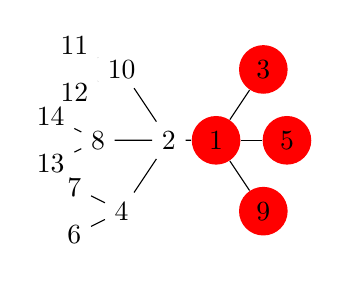
\begin{tikzpicture}[scale = 0.3]
  [scale=0.8,auto=left,every node/.style={circle,fill=sotonblue!20}]

  \node[style={circle,fill=red!100}] (n1) at (7,5) {1};
  \node (n2) at (5,5)  {2};
  \node[style={circle,fill=red!100}] (n3) at (9,8)  {3};
  \node (n4) at (3,2) {4};
  \node[style={circle,fill=red!100}] (n5) at (10,5)  {5};
  \node (n6) at (1,1)  {6};
  \node (n7) at (1,3)  {7};
  \node (n8) at (2,5)  {8};
  \node[style={circle,fill=red!100}] (n9) at (9,2)  {9};considering
  \node (n10) at (3,8)  {10};
  \node (n11) at (1,9)  {11};
  \node (n12) at (1,7)  {12};
  \node (n13) at (0,4)  {13};
  \node (n14) at (0,6)  {14};
  \foreach \from/\to in {n1/n2,n1/n3,n1/n5,n1/n9,n2/n4,n2/n8,n2/n10,n10/n11,n10/n12,n8/n14,n8/n13,n4/n7,n4/n6}
    \draw (\from) -- (\to);
\end{tikzpicture}
\caption{}\label{fig2}
\end{figure}
\end{frame}

\begin{frame}{What we did}
We used  \emph{matlab} to build a model which replicates CAA.  The model is constituted of four processes:
\begin{itemize}
\item[(i)]Generate a binary tree, $T_{n}$, on $n$ nodes.
\item[(ii)]Calculate $|Aut(T_{n})|$.
\item[(iii)]Dynamically remove edges of $T_{n}$ according to a predetermined probability model.
\item[(iv)]Record the time, $\tau_{\frac{1}{2}}$, to remove half of the edges from $T_{n}$ which we think of as the "half-life" of the process.
\end{itemize} 

\end{frame}

\begin{frame}{The Model of cerebral vasculature}
We built a tree, $T$ such that:
\begin{itemize}
 \item[] $T$ has 300 vertices and maximum degree 2.
 \item[] We associate each edge in $T$ with an annular prism.
 \item[]We know the cross-sectional area of edges (corresponding to a capillaries) and every other edge's cross-sectional area can be derived from    Murray's law adjusted for annular prisms.
 \[r_{p}^{3} = r_{d1}^{3} + r_{d2}^{3}\]
  \item[]So we know the volume, $Vol(e)$, of any edge $e \in E(T)$.
 \end{itemize}


\end{frame}

\begin{frame}{The Model of CAA}
\begin{itemize}
 \item[]At time $t=0$ we set $T(0)$ to be our randomly generated binary tree.

 \item[]At time  $t = 1,2,\dots$ for every edge we build $T(t)$ from $T(t-1)$ by defining a probability, $P$, that each edge is removed. Where $P$ is defined in terms of concentration.
 \item[]We assume that A$\beta$ is produced at an approximately constant rate over our life time and that perivascular drainage is able to remove a constant quantity of $A\beta$ even in the face of adversity (the blockage of certain routes)
 \item[]We define the concentration, $C(t)$, at time $t$ to be $\frac{\text{initial volume}}{\text{current volume}}$.   
 \item[]If edge $e = e_{uv}$ is removed then we also remove all branches further away from  the root than $e_{uv}$.  
 \end{itemize}
\end{frame}

\begin{frame}{Results}

The mean half-life of the generated trees.

\begin{figure}[H]
              \centering
            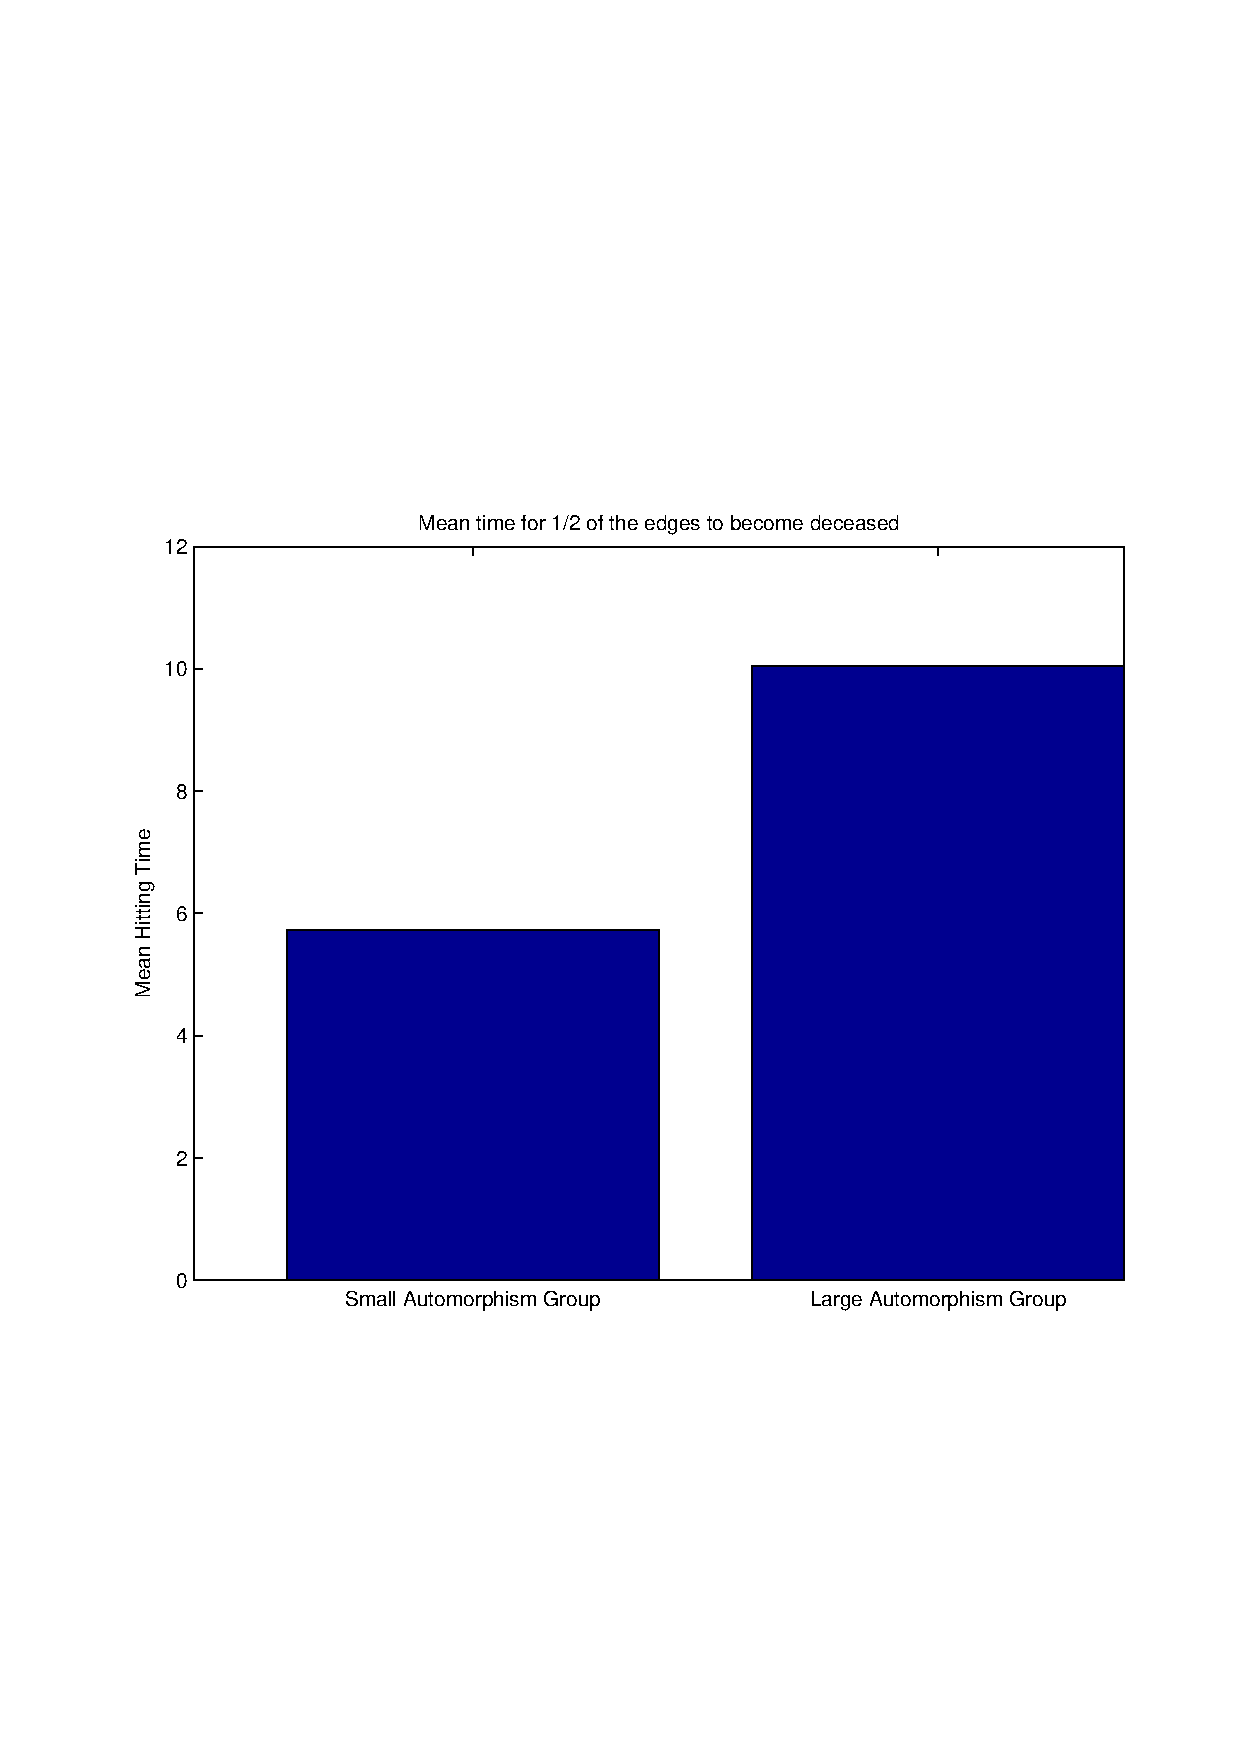
\includegraphics[scale=0.3]{halof.pdf}
                \caption{$\tau_{\frac{1}{2}}$.}\label{t12}
\end{figure}
\end{frame}

\begin{frame}{An extreme example}


\begin{figure}[H]
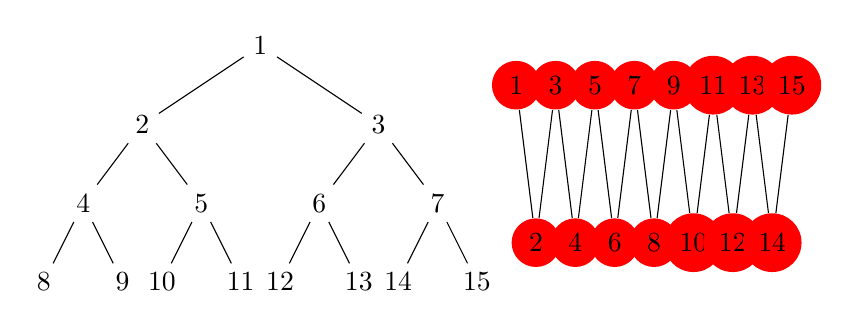
\begin{tikzpicture}[scale=0.5]
  [scale=0.9,auto=left,every node/.style={circle,fill=blue!20}]
  \node (n1) at (5.5,7) {1};
  \node (n2) at (2.5,5)  {2};
  \node (n3) at (8.5,5)  {3};
  \node (n4) at (1,3) {4};
  \node (n5) at (4,3)  {5};
  \node (n6) at (7,3)  {6};
\node (n7) at (10,3)  {7};
\node (n8) at (0,1)  {8};
\node (n9) at (2,1)  {9};
\node (n10) at (3,1)  {10};
\node (n11) at (5,1)  {11};
\node (n12) at (6,1)  {12};
\node (n13) at (8,1)  {13};
\node (n14) at (9,1)  {14};
\node (n15) at (11,1)  {15};

\node[style={circle,fill=red!100}] (n16) at (12,6)  {1};
\node[style={circle,fill=red!100}] (n17) at (12.5,2)  {2};
\node[style={circle,fill=red!100}] (n18) at (13,6)  {3};
\node[style={circle,fill=red!100}] (n19) at (13.5,2)  {4};
\node[style={circle,fill=red!100}] (n20) at (14,6)  {5};
\node[style={circle,fill=red!100}] (n21) at (14.5,2)  {6};
\node[style={circle,fill=red!100}] (n22) at (15,6)  {7};
\node[style={circle,fill=red!100}] (n23) at (15.5,2)  {8};
\node[style={circle,fill=red!100}] (n24) at (16,6)  {9};
\node[style={circle,fill=red!100}] (n25) at (16.5,2)  {10};
\node[style={circle,fill=red!100}] (n26) at (17,6)  {11};
\node[style={circle,fill=red!100}] (n27) at (17.5,2)  {12};
\node[style={circle,fill=red!100}] (n28) at (18,6)  {13};
\node[style={circle,fill=red!100}] (n29) at (18.5,2)  {14};
\node[style={circle,fill=red!100}] (n30) at (19,6)  {15};

  \foreach \from/\to in {n1/n2,n1/n3,n2/n4,n2/n5,n3/n6,n3/n7,n4/n8,n4/n9,n5/n10,n5/n11,n6/n12,n6/n13,n7/n14,n7/n15,n16/n17,n17/n18,n18/n19,n19/n20,n20/n21,n21/n22,n22/n23,n23/n24,n24/n25,n25/n26,n26/n27,n27/n28,n28/n29,n29/n30}
    \draw (\from) -- (\to);

\end{tikzpicture}
%\caption{$T_{1}$ and $T_{2}$}\label{fig:silly}
\end{figure}
\begin{align}
\text{Expected time to remove edges from $G_{1}$: }& 1\frac{8}{14} + 3\frac{4}{14} + 7\frac{2}{14} = \frac{12}{7} \\
%\end{equation} 
%\begin{equation}
\text{Expected time to remove edges from $G_{2}$: }&\frac{1}{14}\sum_{k=1}^{14}k = \frac{15}{2} > \frac{12}{7}
\end{align}
\end{frame}



\begin{frame}{Future Work}
In order to improve the accuracy of our model we could make several modifications:
\begin{itemize}
 \item[(i)] Account for angiogenisis.
 \item[(ii)] Fine tune the CAA deletion of node process. 
 \item[(iii)] Take into account the tortuous routes of perivascular drainage / the stiffening of arteries over time.
 
\end{itemize}

We also wish to verify the result by providing experimental evidence.  
%e.g. Further evidence of this correlation could be found by examining the relationship between highly symmetric areas of the brain and the extent to which those areas are affected by CAA.


\end{frame}

\begin{frame}{Comments and Questions}

\end{frame}
\end{document}



\end{document}